\chapter{Quantum Computing Fundamentals}

\section{Principles of Quantum Mechanics}
Quantum computing is based on key quantum principles:

\begin{itemize}
    \item \textbf{Superposition:} Quantum bits (qubits) can exist in multiple states simultaneously, unlike classical bits that are either 0 or 1.
    
    \item \textbf{Entanglement:} Two or more qubits can become correlated in ways that have no classical equivalent, allowing changes to one qubit to instantly affect another regardless of distance.
    
    \item \textbf{Measurement:} Observing a quantum system causes its superposition to collapse to a single state, with the outcome being probabilistic.
\end{itemize}

\section{Quantum Bits (Qubits)}
Qubits are the fundamental units of quantum information. While a classical bit is binary (0 or 1), a qubit can exist in a superposition of both states, represented as:

\begin{equation}
|\psi\rangle = \alpha|0\rangle + \beta|1\rangle
\end{equation}

where $\alpha$ and $\beta$ are complex numbers satisfying $|\alpha|^2 + |\beta|^2 = 1$.

\section{Quantum Gates and Circuits}
Quantum computation uses quantum gates to manipulate qubits. Basic gates include:

\begin{itemize}
    \item \textbf{Hadamard (H) Gate:} Creates superposition by transforming $|0\rangle$ into $\frac{|0\rangle + |1\rangle}{\sqrt{2}}$
    
    \item \textbf{Pauli Gates (X, Y, Z):} Perform basic rotations on the Bloch sphere
    
    \item \textbf{CNOT Gate:} A two-qubit gate that flips the second qubit if the first is $|1\rangle$
\end{itemize}

% Temporarily commenting out problematic image - replace with actual PNG file later
% \begin{figure}[h]
%     \centering
%     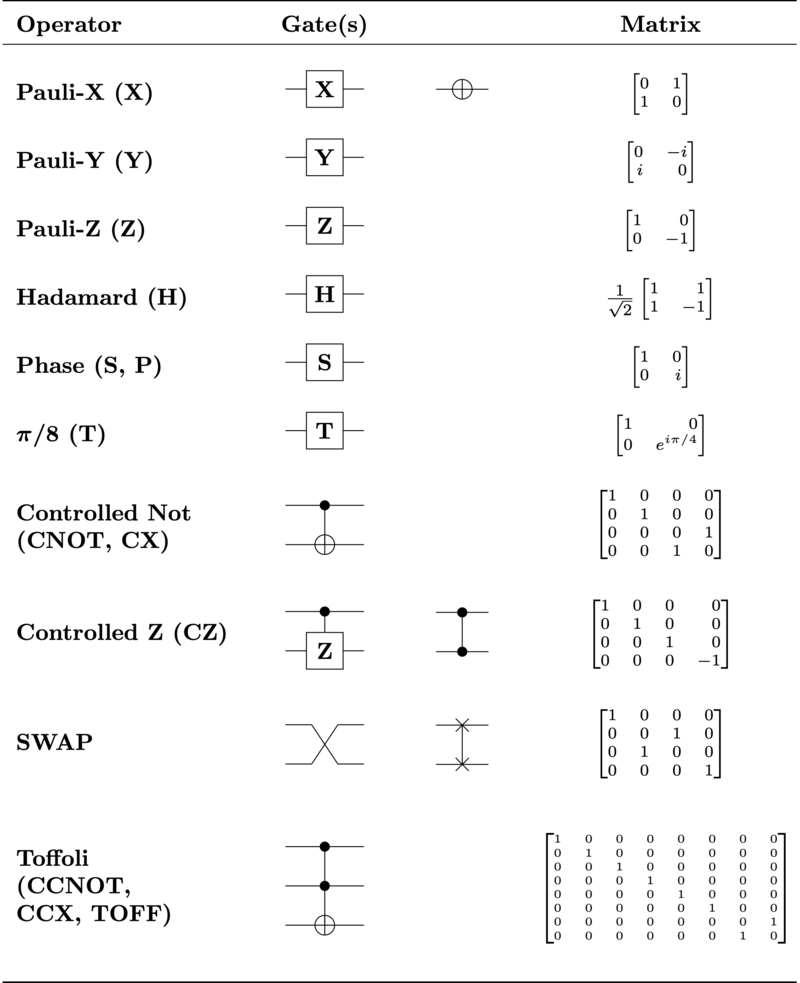
\includegraphics[width=0.6\textwidth]{src/images/quantum_gates.png}
%     \caption{Common Quantum Gates}
% \end{figure}

\section{Quantum Algorithms}
Quantum computers can solve certain problems more efficiently than classical computers:

\begin{itemize}
    \item \textbf{Shor's Algorithm:} Exponentially faster factorization of large numbers, threatening RSA encryption
    
    \item \textbf{Grover's Algorithm:} Provides quadratic speedup for unstructured search problems
\end{itemize}

% Temporarily commenting out problematic image - replace with actual PNG file later
% \begin{figure}[h]
%     \centering
%     \includegraphics[width=0.7\textwidth]{src/images/shor_algorithm.png}
%     \caption{Overview of Shor's Algorithm}
% \end{figure}

\section{Quantum Computing Models}
Several quantum computing approaches exist:

\begin{itemize}
    \item \textbf{Gate-based quantum computing:} Uses quantum circuits with sequences of gates
    
    \item \textbf{Quantum annealing:} Finds the minimum energy state of a system, suited for optimization problems
\end{itemize}

\section{Current State of Quantum Computing}
Current quantum computers are in the Noisy Intermediate-Scale Quantum (NISQ) era:

\begin{itemize}
    \item Limited number of qubits (50-100 range)
    \item Short coherence times
    \item High error rates requiring error correction
\end{itemize}

While not yet able to break cryptographic systems, progress is rapid, with government and industry investing heavily in quantum technology development.